\documentclass[journal, a4paper]{IEEEtran}

\usepackage{graphicx}
\usepackage{url}
\usepackage{bm}
\usepackage{amsmath}
\usepackage[justification=centering]{caption}
% Your document starts here!
\begin{document}
\begin{titlepage}

\newcommand{\HRule}{\rule{\linewidth}{0.5mm}} % Defines a new command for the horizontal lines, change thickness here

\center % Center everything on the page
 %----------------------------------------------------------------------------------------
%	LOGO SECTION
%----------------------------------------------------------------------------------------

~\\[1cm]

\includegraphics{SCUT.png}\\[2cm] % Include a department/university logo - this will require the graphicx package

%----------------------------------------------------------------------------------------
%	TITLE SECTION
%----------------------------------------------------------------------------------------

\HRule \\[1cm]
{ \huge \bfseries The Experiment Report of \textit{Deep Learning} }\\[0.6cm] % Title of your document
\HRule \\[2cm]
%----------------------------------------------------------------------------------------
%	HEADING SECTIONS
%----------------------------------------------------------------------------------------


\textsc{\LARGE \textbf{School:} School of Software Engineering}\\[1cm]
\textsc{\LARGE \textbf{Subject:} Software Engineering}\\[2cm]


%----------------------------------------------------------------------------------------
%	AUTHOR SECTION
%----------------------------------------------------------------------------------------

\begin{minipage}{0.4\textwidth}
\begin{flushleft} \large
\emph{Author:}\\
Qichen Huang % Your name
\end{flushleft}
\end{minipage}
~
\begin{minipage}{0.4\textwidth}
\begin{flushright} \large
\emph{Supervisor:} \\
Mingkui Tan% Supervisor's Name
\end{flushright}
\end{minipage}\\[2cm]
~
\begin{minipage}{0.4\textwidth}
\begin{flushleft} \large
\emph{Student ID:}\\
201920142806
\end{flushleft}
\end{minipage}
~
\begin{minipage}{0.4\textwidth}
\begin{flushright} \large
\emph{Grade:} \\
Graduate
\end{flushright}
\end{minipage}\\[2cm]

% If you don't want a supervisor, uncomment the two lines below and remove the section above
%\Large \emph{Author:}\\
%John \textsc{Smith}\\[3cm] % Your name

%----------------------------------------------------------------------------------------
%	DATE SECTION
%----------------------------------------------------------------------------------------

{\large \today}\\[2cm] % Date, change the \today to a set date if you want to be precise


%----------------------------------------------------------------------------------------

\vfill % Fill the rest of the page with whitespace

\end{titlepage}

% Define document title and author
	\title{Linear Regression and Stochastic Gradient Descent}
	\maketitle

% Write abstract here
\begin{abstract}
Linear Regression is to find a linear function that can predict a continuous value properly. We carry out this experiment to reveal the theory and implementation details of linear regression. The experiment is conducted via Close-Form Solution and Stochastic Gradient descent. Both of them produce promising results.
\end{abstract}

% Each section begins with a \section{title} command
\section{Introduction}
	% \PARstart{}{} creates a tall first letter for this first paragraph
\IEEEPARstart{R}{egression} is one of the most common problem in Machine Learning, which is to make up a function mapping from specific features to a continuous value, named label. Its linear situation brings out a certain version, called Linear Regression. In this experiment, we attempt to figure out the theory of Linear Regression and reveal details of its implementation. Our motivation is to 1) understand Linear Regression and its implementation, both close-form solution and stochastic gradient descent solution, 2) conduct some experiments under small scale dataset, 3) experience the process of optimization, like adjusting parameters. We conduct experiments on Housing Data in LIBSVM, with close-form and stochastic gradient descent. Both of them give out promising result.

% Main Part
\section{Methods and Theory}
The target of Linear Regression is to find a linear function $\hat{y_i}=\bm{x}_i^T\bm{w}+b$ so that for every single feature data $\bm{x}_i$, its predicted value $\hat{y_i}$ gets as close to the ground truth value $y_i$ as possible, in which $\bm{x}_i$ and $\bm{w}$ are both column vectors. Thus the only effort is to search proper value for parameter $\bm{w}$ and $b$. To conveniently solve this problem, we define a loss function $\mathcal{L}_i=\frac{1}{2}(y_i-\hat{y_i})^2$ for $i$ th feature data to calculate the difference between $y_i$ and $\hat{y_i}$. As a result, the total loss function is $\mathcal{L}=\frac{1}{2}\sum_i{(y_i-\hat{y_i})^2}$. With matrix representation, it can be written as $\mathcal{L}=\frac{1}{2}(Y-\hat{Y})^T(Y-\hat{Y})$ where $Y$ and $\hat{Y}$ are batch ground truth and batch predicted value separately, and both of them are column vectors. After that, the parameter searching problem is converted to minimization problem of loss function. In this experiment, the minimization problem is solved with close-form solution and stochastic gradient descent.
\subsection{Close-Form Solution}
As the loss function of Linear Regression is convex, the minimum of function can be reached by setting its derivative to zero. For convenience of calculation, we absorb parameter $b$ into $\bm{w}$ and append $1$ to the end of every feature data $\bm{x}_i$. Then the batch predicted value $\hat{Y}$ can be computed as $\hat{Y}=X\bm{w}$, where $X=\{\bm{x}_1^T,\bm{x}_2^T,...,\bm{x}_n^T\}^T$ is batch feature data. After setting derivative of loss function $-X^TY+X^TX\bm{w}$ to zero, we can get $w=(X^TX)^{-1}X^TY$.
\subsection{Stochastic Gradient Descent}
Gradient, vector of partial derivative, points in the direction of greatest increase of a function. In other words, negative gradient points to the greatest decrease of function. That is to say, if we update parameters of loss function towards negative gradient direction, the loss function will get to minimum. This is the idea behind Gradient Descent. However, both Close-Form Solution and Gradient Descent face the problem in which computation involving the whole batch of data might use out of memory and fails to output final result. As an alternative Stochastic Gradient Descent considers updating parameters with gradient computed from only single data. For data $(\bm{x}_i,y_i)$, we can compute gradient as $\mathcal{G}_i=(\bm{w}^T\bm{x}_i-y_i)\bm{x}_i$. Then $\bm{w}$ is updated as $\bm{w}=\bm{w}-\eta\mathcal{G}$, where $\eta$ is the learning rate.

\section{Experiments}
\subsection{Dataset}
The experiments use scaled Housing Data in LIBSVM which includes 506 samples and each sample has 13 features. These samples are further divided into training set, $\frac{2}{3}$ of total, and validation set, $\frac{1}{3}$ of total.
\subsection{Implementation}
\subsubsection{Experiment Step}
For Close-Form Solution, the experiment steps are as follows:
\begin{enumerate}
  \item Load the experiment data.
  \item Divide dataset into training set and validation set.
  \item Select a loss function
  \item Get the formula of the Close-Form Solution.
  \item Get the value of parameter \textit{W} by the Closed-Form Solution, and update the parameter \textit{W}.
  \item Get the \textit{loss}, \textit{loss\_train} under the training set and \textit{loss\_val} by validating under validation set.
  \item Output the value \textit{loss}, \textit{loss\_train} and \textit{loss\_val}.
\end{enumerate}
For Stochastic Gradient Descent, the experiment steps are as follows:
\begin{enumerate}
  \item Load the experiment data.
  \item Divide dataset into training set and validation set.
  \item Initialize linear model parameters.
  \item Choose loss function and derivative.
  \item Calculate gradient \textit{G} toward loss function from each sample.
  \item Denote the opposite direction of gradient \textit{G} as \textit{D}.
  \item Update model:$W_t=W_{t-1}+\eta D$. $\eta$ is learning rate, a hyper-parameter that we can adjust
  \item Get the \textit{loss\_train} under the training set and \textit{loss\_val} by validating under validation set.
  \item Repeat step 5 to 8 for several times, and output the value of \textit{loss\_train} as well as \textit{loss\_val}.
\end{enumerate}
\subsubsection{Initialization}
In Close-Form Solution, no parameters need to be initialized. While in Stochastic Gradient Descent, $\bm{w}$ is initialized randomly. Learning rate and training step are initialized to 0.01 and 10000 separately.
\subsubsection{result}
The final result of experiments are presented in Table \ref{tab:result} and training process of Stochastic Gradient Descent is depicted in Fig. \ref{fig:training_process}.

\begin{table}[!hbt]
\begin{center}
\caption{Experiment Result}
\label{tab:result}
\begin{tabular}{c|cc}
  \hline
  Loss & training loss & validation loss \\
  \hline
  Close-Form Solution & 11.492508 & 10.362012 \\
  Stochastic Gradient Descent & 11.786695 & 10.534759 \\
  \hline
\end{tabular}
\end{center}
\end{table}

\begin{figure}[!hbt]
\begin{center}
    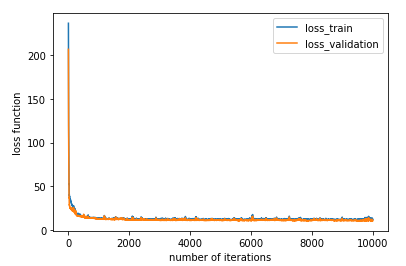
\includegraphics[width=\columnwidth]{training_process_of_SGD}
    \caption{Training Process of SGD}
    \label{fig:training_process}
\end{center}
\end{figure}

\section{Conclusion}
In this experiment, we explored linear regression problem with Close-Form Solution and Stochastic Gradient Descent. Because the loss function of linear function is convex, Close-Form Solution reaches the minimum, which is better than Stochastic Gradient Descent. Although Stochastic Gradient Descent can perfectly handle out-of-memory problem, it also results in fluctuation during training process, slowing down the optimization.



% Your document ends here!
\end{document}
